\documentclass[tikz,border=2pt]{standalone}
\usepackage{amsmath}
\usepackage{pgfplots}
\pgfplotsset{compat=1.18}
\usetikzlibrary{arrows.meta}
\begin{document}
% Continuous life annuity at rate 100, lambda = 0.02, delta = 0.03: the survival-weighted discounted
% rate is 100 v^t {}_tp_x = 100 e^{-0.05t}, and the area under it is the APV 100/0.05 = 2000.
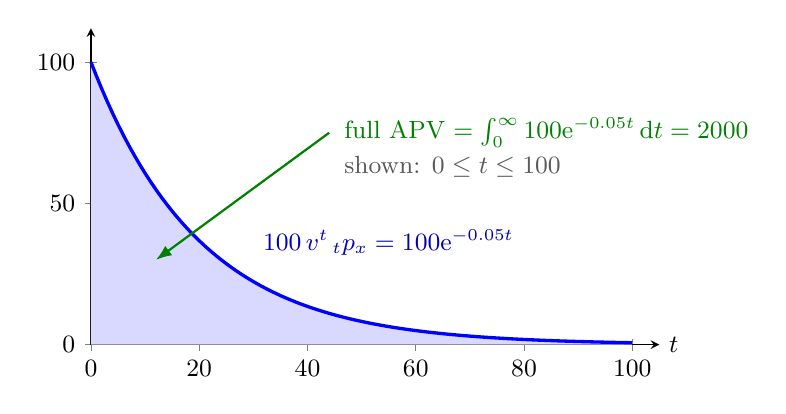
\begin{tikzpicture}[font=\small, >={Latex[length=2mm]}]
  \begin{axis}[
    axis lines=left, xmin=0, xmax=105, ymin=0, ymax=112,
    xtick={0,20,40,60,80,100}, ytick={0,50,100},
    xlabel={$t$},
    xlabel style={at={(axis description cs:1,0)}, anchor=west},
    samples=100, width=8.8cm, height=5.6cm, clip=false]
    \addplot[fill=blue!15, draw=none, domain=0:100] {100*exp(-0.05*x)} \closedcycle;
    \addplot[blue, very thick, domain=0:100] {100*exp(-0.05*x)};
    \node[blue!70!black, anchor=south west] at (axis cs:30,28) {$100\,v^t\,{}_tp_x=100\mathrm{e}^{-0.05t}$};
    \draw[->, green!50!black, thick] (axis cs:44,75) -- (axis cs:12,30);
    \node[green!50!black, anchor=west] at (axis cs:45,75) {full APV $=\int_0^\infty100\mathrm{e}^{-0.05t}\,\mathrm{d}t=2000$};
    \node[gray!70!black, anchor=west] at (axis cs:45,63) {shown: $0\le t\le100$};
  \end{axis}
\end{tikzpicture}
\end{document}
